
\chapter{Description of the developed functionalities}
This chapter will give a description of the functionalities that are developed for our application. The requirements mentioned in the introduction are used to reflect on the functionalities.
\section{Semantic zooming}
\begin{wrapfigure}{r}{0.2\textwidth}
	\centering
	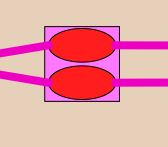
\includegraphics{images/mutation.jpg}
	\caption{\label{fig:bubble}A mutation bubble}
\end{wrapfigure}
Semantic zooming should be provided to the customer which initially shows the entire graph, and on which the user can zoom in to see more details. This is implemented by making bubbles, which collapse nodes together, and showing these at a high-level view. When zooming in (which happens stepless), the bubbles are expanded and more details of the graph are shown. By creating bubbles, large amounts of genomes can be visualized. When nodes in the graph (which represent base sequences) are big enough they become visible. Figure X+1 shows an example of a bubble (the purple square), containing two nodes, which has been expanded. 

\section{Phylogenetic tree}

\begin{wrapfigure}{l}{5cm}
	\centering
	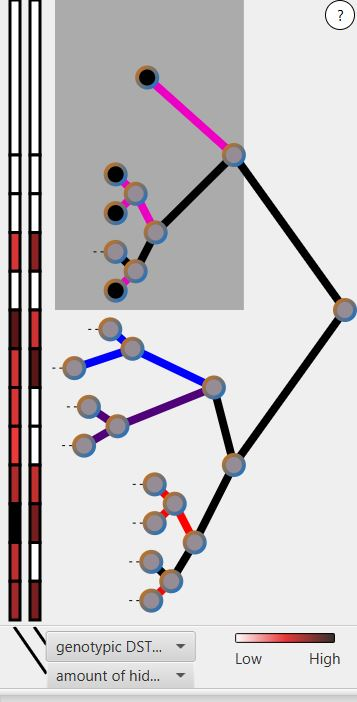
\includegraphics[width=0.3\textwidth]{images/tree.jpg}
	\caption{\label{fig:tree}The phylogenetic\\tree}
\end{wrapfigure}

The phylogenetic tree can be used to visualize a subset of the genomes. The tree in the application can be zoomed in on, because not every leaf node can be shown on the screen when the dataset is big. By zooming in, nodes on a deeper level become visible. 
\par
There exist lineages in the phylogeny, which is a grouping of genomes. These lineages have a specific colour which is shown on the edges between nodes in the tree. 
\par
On the left of the tree is a heatmap which can be used to show the density of properties of the tree (e.g. the number of leaf nodes in a certain branch). 
\par
Nodes can be dragged from the phylogenetic tree to the main graph area and all genomes contained in the leaves of the selected tree are then drawn on the screen. When dragged to the main area a popup will appear asking if the genomes should be added to the existing graph, if a new graph has to be created, or if the specific nodes have to be removed from the current visualization. 
\par
Because the application builds on the idea that the comparison of two graphs can be useful, two graphs can be drawn on the main screen. Nodes in the tree have colouring to indicate in which graph(s) they are present. There is a legend present for all visuals in the tree. 
Figure X+2 shows an example of the phylogenetic tree, with one heatmap containing the amount of hidden nodes in a branch and the other heatmap containing the amount of genotype DST:XDR in a branch.
\section{The main area}
The main area is the part where the graph is drawn. As mentioned before, there can be a graph on the top half and a graph on the bottom half (see figure X). It is also possible to show only one graph. Loading is performed with simple dragging and dropping from the phylogenetic tree. When a graph is loaded, the user sees different rectangles, ellipses, and colours. These represent different types of bubbles, which are explained in the legend. 
\section{Searching}
On the main screen a searching pane is available. A search can be performed based on metadata about the genomes. Multiple genomes that resulted from a search can be selected and dragged to the main graph. This works the same as dragging and dropping from the phylogenetic tree.
\section{Loading}
When the application is started a file loader appears wherein the files to be loaded can be selected. The application supports the .gfa file-format for the graph, the .nwk file-format for the phylogenetic tree, the .gff file-format for the annotations and the .xlsx file-format for the metadata. 
\section{Settings}
There is a settings menu, where the user can select which bubbling algorithms it wants to use (if any). There are five options to choose from, which are explained in the application.